\section{Implementation}
The group has chosen system prototyping as the primary methodology of the study Fig. ~\ref{fig:SPD}. It is effective to use this because Arduino is quick to learn and would be useful in creating prototypes easily. It will also be advantageous to follow this methodology because of the time constraint and weekly updates. This would, however, not be very effective in terms of developing an Android application with a crowdsourcing element and bluetooth communications due to its unfamiliarity to the group. 

\begin{figure}[h]
	\centering
	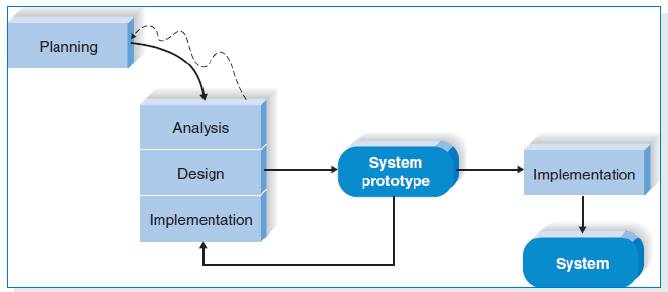
\includegraphics[width=\textwidth]{GraphColor}
	\caption{System Prototyping Diagram}
	\label{fig:SPD}
\end{figure}

\subsection{Planning}
The planning stage took around four weeks. In the planning stage, several factors of air quality was taken into consideration. Among these factors are temperature, humidity, dust, and amount of Carbon Monoxide. In creating this design, few more considerations must be accounted for. Among these are portability, Android compatibility, and real time. Different stages must take place in creating the proposed system. These stages will consist of the integration of the different sensors to our design, testing and evaluating these sensors, and integrating them in the Android application. 

\subsection{Initial Prototype}
For the initial prototype, the temperature and humidity are first taken into consideration. The design will include the DHT11 humidity sensor and an LED display to provide feedback on the current temperature and humidity as well as the discomfort index of the area. Several sets of data are first taken in order to retrieve the temperature and humidity. This is done in order to a check the consistency and accuracy of the measuring devices used for comparing the data collected from our design. The data is taken from 3 different days with 2 analog and 1 digital sensor. The prototype will make use of the DHT11 sensor and and its accuracy will be tested using the best thermometer and hygrometer.

\subsection{Second Prototype}
More features are added in the initial prototype.These will include bluetooth communications with the Android app as well as integrating crowdsourcing using FireBase. This will also include the SDS011 particulate matter laser sensor which measures the concentration of dust present locally. The use of this sensor will have a relative error of 10\% . This error will be tested by comparing the results to a DustTrak or GRIMM dust monitor.

\subsection{Final Prototype} 
Using  MQ-7 CO sensor, the prototype will be further extended. The range will be from 10 to 500 ppm which is sufficient to determine how harmful the amount is. This too will be compared to an existing CO meter which will be used to measure the reliability of the sensor. The final prototype will also include the integration of visibility detection. The visibility detection will make use of OpenCV by making use of Canny Edge Detection. The prototype will also finalize the Android application's features and design.

\subsection{Integration of Communication Devices}
The data transferred will not only be transferred to the proposed Android application but also to a cloud. This will involve crowdsourcing which would enable several data to be inputted at real time. To transfer the data from the proposed system to the Android application, the SMiRF Bluetooth module or HC-05 Bluetooth module will be used. The data collected will then be transferred to a Firebase database. 

\section{Evaluation}

The study is to develop a mobile phone application that utilizes the use of a microcontroller-based system to measure air parameters in getting the discomfort index and amount of air pollutants. The discomfort index is dependent on air parameters measured by the system. In relation to the air parameters, the study uses a quantitative approach of data gathering, through actual measurements of air parameters using analog and digital meters and sensors. A crowdsourcing approach was then applied for better information gathering between the users of the applications across the map. 

\subsection{Quantitative Approach}
Data were gathered four nonconsecutive trials on twenty different locations along De La Salle University. The data collected is consists of the measurements of the available meters, one digital and two analog meters, and the measurements of the actual sensors used on the system. The time and date, when the data were taken, were also recorded due to the fact that the parameters greatly varies on the weather and the time it was measured which also leads to inconsistent recorded data. 

The gathered data were used to determine the reliability of the measurements from the sensors used in the system, in resemblance to the measurements from the meters. The use of the meters are for establishing the ground truth of the measurements of air parameters. Also, the data were ranked according to their corresponding computed level of discomfort or discomfort index based on the parameters measured using both the meters and the sensors.

\subsection{Crowdsourcing Approach}
Due to the fact that the data can only be collected when the user is at the specified location, the android application used in this study integrates a crowdsourcing approach in gathering of data. In this way, the user can be aware of the conditions of the air parameters around a location on the map based on the data from the other users that are in the location. 

The application is capable of sharing or storing information in a cloud for crowdsourcing. The cloud is used to hold the data from all the information stored by each users of the application. The crowdsourcing application is very dependent on the users data and it would be most effective when more people uses the application. This approach allows the user to gather information and at the same time, contributes to the cloud-based system of the application which also contributes to the data gathering of other users.

\section{Summary}
The proposed design will contain several sensors that will measure temperature, humidity, particulate matter amount, and levels of carbon dioxide. There are different stages in gathering the various data required. The sensors will be calibrated based from its individual datasheets. The data will be taken in a span of two weeks and at different times throughout the day. The data taken from our design will be compared with commercial sensors that are readily available to test the reliability and consistency of the proposed design. 

The data collected from DHT11 sensor for detecting temperature and humidity will be measured. The design will also use a SDS011 PM laser sensor to record the amount of dust present within its range. The MQ-7 CO sensor will record the concentrations of Carbon Monoxide in its vicinity. The range will be from 10 to 500 ppm which is sufficient to determine how harmful the amount of Carbon Monoxide is. These will be tested with their corresponding meters and its accuracy will be determined. The data collected will be sent to a database in a cloud and transferred to the Android application. The program within the application will handle the discomfort index calculation and will determine level of discomfort.


